\begin{enumerate}[label=\thesubsection.\arabic*.,ref=\thesubsection.\theenumi]
\numberwithin{equation}{enumi}
\item An op amp with an open loop voltage gain of 80dB and poles at $10^{5}$Hz , $10^{6}$ Hz and $2\times10^{6}$ Hz is said to be compensated to be stable for unity $\beta$. Assume that op amp incorporates an amplifier circuit equivalent to Fig.\ref{fig:Eqivalent circuit }  with $C_{1}$=150pF ,$C_{2}$=5pF and $g_{m}$=40mA/V and that $f_{p1}$ is caused by input circuit and $f_{p2}$ by the output circuit of this amplifier.Find the required value of compensating miller capacitance and the new frequency of the output pole

\begin{figure}[h!]
	\begin{center}
		\resizebox{\columnwidth/1}{!}{\begin{circuitikz}[american]
\ctikzset{tripoles/mos style/arrows}
\draw  (0,0) node[ground](GND){} -- (0,1) to[isource, l= $I_{i}$] (0,3) -- (1,3);
\draw (1,3) to[R=$R_{1}$] (1,0) node[ground](GND){};
\draw (1,3) node[label={B}]{} to[short] (3,3);
\draw (2,1.8) node[label=$+$]{}; 
\draw (2,0.3) node[label=$-$]{};
\draw (2,1) node[label=$V_{0}$]{}; 
\draw (3,3) to[C=$C_{1}$] (3,0) node[ground](GND){};
\draw (3,3) node[]{} to[short] (3.5,3);
\draw (3.5,3) to[C=$C_{f}$] (5.5,3);
\draw (5.5,3) to[cisource, l= $g_{m_{2}}V_{0}$] (5.5,0) node[ground](GND){};
\draw (5.5,3) node[label={C}]{} to[short] (7.3,3);
\draw (7.3,3) to[R=$R_{2}$] (7.3,0) node[ground](GND){};
\draw (7.3,3) node[]{} to[short] (8.5,3);
\draw (8.5,3) to[C=$C_{2}$] (8.5,0) node[ground](GND){};

\end{circuitikz}
}
	\end{center}
	\caption{Equivalent amplifier circuit}
	\label{fig:Eqivalent circuit }
\end{figure}

\solution

The analysis of the circuit yields the transfer function
\begin{multline}
    \frac{V_{0}}{I_{i}} = \frac{\brak{sC_{f}-g_{m}}R_{1}R_{2}}{1+s\sbrak{P}+s^{2}\sbrak{Q}}
    \label{eq:ee18btech11029_1}
\end{multline}
where
\begin{align}
    P&={C_{1}R_{1}+C_{2}R_{2}+C_{f}\brak{g_{m}R_{1}R_{2}+R_{1}+R_{2}}}\\
    Q&={\brak{C_{1}C_{2}+C_{f}\brak{C_{1}+C_{2}}}R_{1}R_{2}}
\end{align}
The zero is usually at a much higher frequency so neglecting its effect ,the denominator of the transfer function can be written in the form
\begin{align}
    D(s)=\brak{1+\frac{s}{\omega_{p1}^{'}}}\brak{1+\frac{s}{\omega_{p2}^{'}}}
\end{align}
Here $\omega_{p1}^{'}$ and $\omega_{p2}^{'}$ are the new frequencies of the two poles and one of the pole will be dominant
\begin{align}
    \omega_{p1}^{'} < \omega_{p2}^{'}
\end{align}
Thus
\begin{align}
    D(s) \approx 1+\frac{s}{\omega_{p1}^{'}}+\frac{s^{2}}{\omega_{p1}^{'} \omega_{p2}^{'}}
    \label{eq:ee18btech11029_2}
\end{align}
Equating the coefficient of s in the Eq. \eqref{eq:ee18btech11029_1} and Eq. \eqref{eq:ee18btech11029_2}
we get
\begin{align}
    \omega_{p1}^{'} = \frac{1}{C_{1}R_{1}+C_{2}R_{2}+C_{f}\brak{g_{m}R_{1}R_{2}+R_{1}+R_{2}}}
\end{align}
This can be approximated to 
\begin{align}
    \omega_{p1}^{'} =\frac{1}{g_{m}R_{1}R_{2}C_{f}}
    \label{eq:ee18btech11029_3}
\end{align}
In order to obtain the value of $\omega_{p2}^{'}$ we equate the coefficient of $s^{2}$ in Eq. \eqref{eq:ee18btech11029_1} and Eq. \eqref{eq:ee18btech11029_2} and use the value of Eq. \eqref{eq:ee18btech11029_3}
\begin{align}
    \omega_{p2}^{'} = \frac{g_{m}C_{f}}{{C_{1}C_{2}+C_{f}\brak{C_{1}+C_{2}}}}
    \label{eq:ee18btech11029_4}
\end{align}

\item Find the value of G
\begin{align}
    80&=20\log\brak{G}\\
    G&=10^{4}
\end{align}
\item Find the values of $R_{1}$ and $R_{2}$\\
\solution The pole $f_{p1}$ is caused by input circuit and $f_{p2}$ by the output circuit.
\begin{align}
    f_{p1} = \frac{1}{2\pi R_{1}C_{1}}\\
    f_{p2} = \frac{1}{2\pi R_{2}C_{2}}
\end{align}
finding the values of $R_{1}$ and $R_{2}$
\begin{align}
     R_{1} &= \frac{1}{2\pi\brak{150\times10^{-12}}\brak{10^{5}}} = 10.61k\Omega
\end{align}
\begin{align}
     R_{2} &= \frac{1}{2\pi\brak{5\times10^{-12}}\brak{10^{6}}} = 31.8k\Omega
\end{align}

Assuming that the pole $f_{p2}$ will move to a frequency $f_{p2}^{'}$. This requires the modified first pole to be located at 
\begin{align}
    f_{p1}^{'} &= \frac{f_{p3}}{G}\\
    &= \frac{2\times10^{6}}{10^{4}} = 200 Hz
\end{align}


\begin{table}[!t]
\centering
\begin{enumerate}[label=\thesubsection.\arabic*.,ref=\thesubsection.\theenumi]
\numberwithin{equation}{enumi}

\item In the block diagram Fig.\ref{fig:ee18btech11029}  
\begin{align}
G\brak{s} = \frac{K}{\brak{s+4}\brak{s+5}}
\label{ee18btech11034_Gs}
\end{align}
\begin{figure}[!ht]
    \begin{center}
		\resizebox{\columnwidth}{!}{\tikzset{
        block/.style = {draw, rectangle,
            minimum height=1cm,
            minimum width=2cm},
        input/.style = {coordinate,node distance=1cm},
        output/.style = {coordinate,node distance=4cm},
        arrow/.style={draw, -latex,node distance=2cm},
        pinstyle/.style = {pin edge={latex-, black,node distance=2cm}},
        sum/.style = {draw, circle, node distance=1cm},
}

\begin{tikzpicture}[node distance=2.5cm,auto,>=latex']
  \node [input, name=input] {};
  \node [sum, right = 1cm of input] (sum) {};
  \node [block, right =0.5 cm of sum] (block1) {$G(s)$};
  \node [sum,right  = 0.7 cm of block1] (sum1){};
  \node [input ,right =0.25cm of block1] (p1) {};
  \node [input ,below = 1 cm of p1] (p2){};
  \node [input ,left = 2.7cm of p2] (p3){};
  \node [input ,above =0.8cm of p3] (p4) {};
  \node [block,right  = 0.5 cm of sum1] (block2) {$G(s)$};
  \node [input ,right =0.25cm of block2] (q1) {};
  \node [input ,below = 1 cm of q1] (q2){};
  \node [input ,left = 2.8cm of q2] (q3){};
  \node [input ,above =0.7cm of q3] (q4) {};
   \node [input ,right =0.8cm of block2] (q5) {};
   \node [input ,below =1.5cm of q5] (q6){};
    \node [input ,left =7.24cm of q6] (q7){};
    \node [input ,above =0.9cm of q7] (q8) {};
    \node [input ,right =1cm of q5] (q9) {};
  
  
  
  
 
  
  
  \draw [->] (input) -- node {$R(s)\ +$} (sum);
  \draw [->] (sum) --  (block1);
 \draw [-]  (block1) -- (sum1);
 \draw [-]  (sum1) -- (block2);
 \draw [-]  (p1) -- (p2);
 \draw [-] (p2) -- (p3);
   \draw [->](p3) -| node[pos=0.90] {$-$} (p4);
  \draw [-] (block2) -- (q1);
  \draw[-] (q1) -- (q2);
  \draw[-] (q2) -- (q3);
  \draw [->](q3) -| node[pos=0.99] {$-$} (q4);
  \draw[-] (block2)--(q5);
   \draw[-] (q5) -- (q6);
    \draw[-] (q6) -- (q7);
  \draw [->](q7) -| node[pos=0.99] {$+$} (q8);
  \draw [->] (q5) -- node {$Y(s)$} (q9);

  %\draw [->] (block1) -- node {} (block2);
%  \draw [->] (block2) -- node [name =y] {$Y(s)$} (output);
 % \draw [->] (y) -- ++ (0,-2) -| node [pos=0.99] {$-$} (sum);

\end{tikzpicture}
}
	\end{center}
\caption{}
\label{fig:ee18btech11029}
\end{figure}
\item Find the range of K for stability by Nyquist criterion

\solution
\begin{figure}[!h]
    \begin{center}
		\resizebox{\columnwidth}{!}{\input{./figs/ee18btech11029/ee18btech11029_2.tex}}
	\end{center}
\caption{}
\label{fig:ee18btech11029_1}
\end{figure}


The open loop transfer function from Fig.\ref{fig:ee18btech11029_1}

\begin{align}
    T\brak{s} =\brak{\frac{\frac{K}{\brak{s+4}\brak{s+5}}}{1+\frac{K}{\brak{s+4}\brak{s+5}}}}^2 
\end{align}


\begin{align}
    T\brak{\j\omega} =\brak{\frac{\frac{K}{\brak{\j\omega+4}\brak{\j\omega+5}}}{1+\frac{K}{\brak{\j\omega+4}\brak{\j\omega+5}}}}^2 
\end{align}




\begin{itemize}
    \item Since it is connected in positive feedback the transfer function cuts at \brak{1,\j0} 
\end{itemize}

\begin{align}
    \implies  \text{Re} \cbrak{T\brak{\j\omega}} &= 1\\
      \implies  \text{Im} \cbrak{T\brak{\j \omega}} &= 0
     \label{eq:ee18btech11029_eq_Re}
\end{align}


\begin{align}
    \brak{\frac{\frac{K}{\brak{\j\omega+4}\brak{\j\omega+5}}}{1+\frac{K}{\brak{\j\omega+4}\brak{\j\omega+5}}}}^2 &= 1+\j0
\end{align}

\begin{align}
    \brak{\j\omega+4}\brak{\j\omega+5}+2K &=0
\end{align}

\begin{align}
    -\omega^2 + 9\j\omega +20+2K &=0 
\end{align}
\\
From  \eqref{eq:ee18btech11029_eq_Re}

\begin{align}
    20 + 2K &= 0\\
    \implies K=-10
\end{align}
The minimum value of stability for the system to be stable is
\begin{align}
    K_{min} > -10
\end{align}
The range of K for which the system is stable is 
\begin{align}
    -10 < K < \infty
\end{align}


\item From the table.\ref{table:ee18btech11029_table1}, 
Stability criterion for K is N+P=Z


\begin{table}[!h]
\centering
\input{./tables/ee18btech11029_table.tex}
\caption{}
\label{table:ee18btech11029_table1}
\end{table}


\item Verify the Nyquist plots by
\begin{lstlisting}
codes/ee18btech11029_1.py
\end{lstlisting}


\begin{figure}[h!]
\centering
  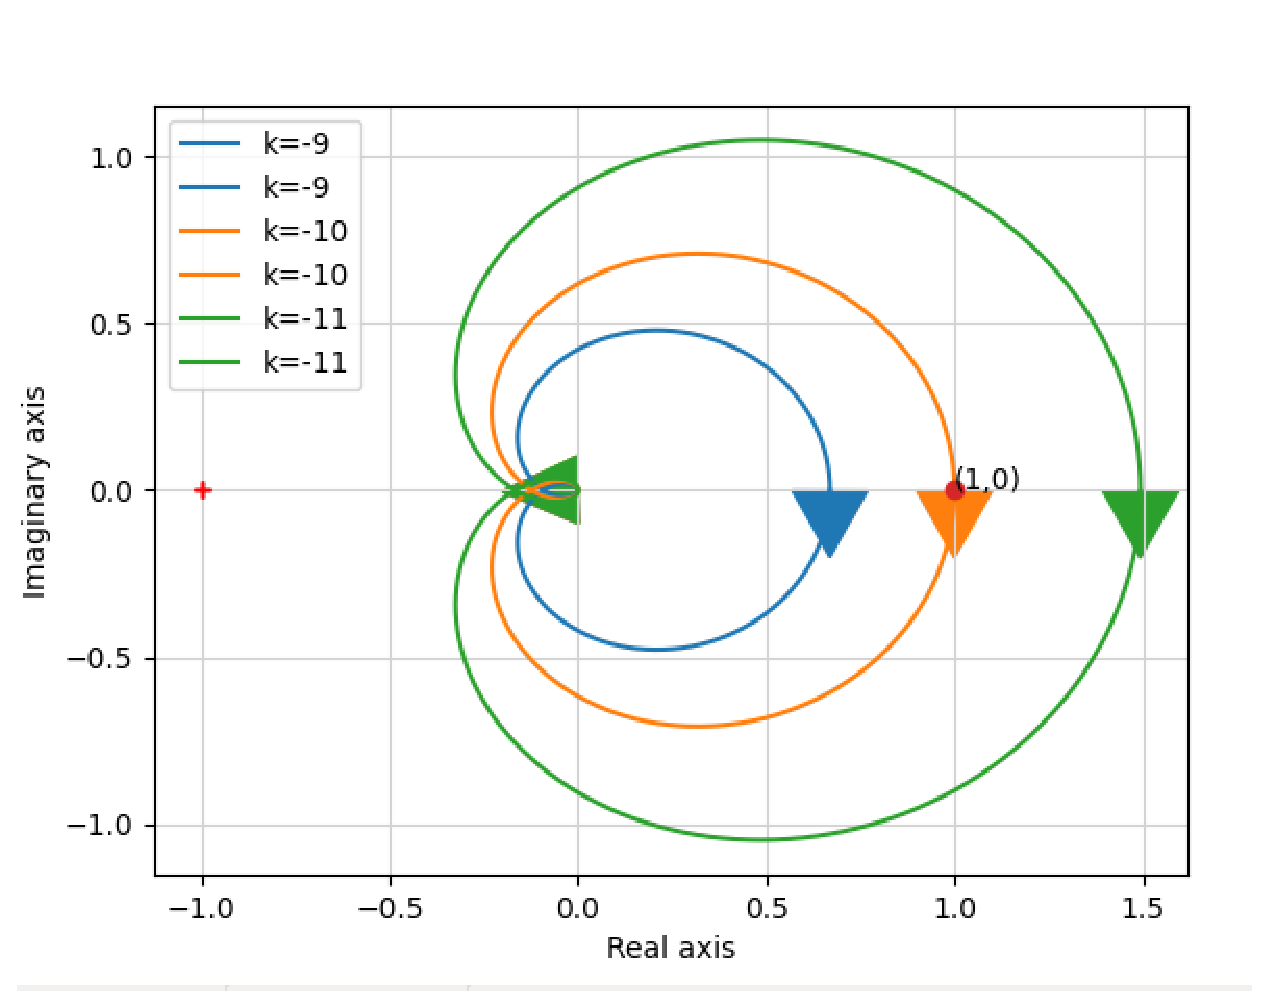
\includegraphics[width=\columnwidth]{./figs/ee18btech11029/Nyquist.eps}
  \caption{Nyquist Plot}
  \label{fig:ee18btech11029_2}
\end{figure}





\item Verify the result using Routh-Hurwitz criterion

\solution The characteristic equation is 
\begin{align}
    1-T\brak{s} &=0\\
    1-\brak{\frac{\frac{K}{\brak{s+4}\brak{s+5}}}{1+\frac{K}{\brak{s+4}\brak{s+5}}}}^2 &=0\\
    1+2\brak{\frac{K}{\brak{s+4}\brak{s+5}}}&=0\\
    s^2+9s+20+2K &= 0
\end{align}

\begin{align}
\mydet{s^2\\s^1\\s^0}
\mydet{1 & 20+2K \\ 9 & 0 \\ 20+2K & 0}
\end{align}
For a system to be stable it should not have any sign changes
\begin{align}
    20+2K >0
\end{align}
This is valid for all positive values of K but the minimum value of K is
\begin{align}
    K>-10
\end{align}
So the range of K for stability is 
\begin{align}
    -10<K<\infty
\end{align}

\item Verify the result by
\begin{lstlisting}
codes/ee18btech11029_2.py
\end{lstlisting}







\end{enumerate}

\caption{}
\label{table: Input_Table}
\end{table}
\item Find the value of Miller capacitance\\
\solution Compensating miller capacitance is 
From Eq.\eqref{eq:ee18btech11029_3} we get
\begin{align}
    C_{f}=\frac{1}{2\pi g_{m}R_{1}R_{2}f_{p1}^{'}}
\end{align}
\begin{align}
    C_{f}&= \frac{1}{2\pi\brak{40\times10^{-3}}\brak{\frac{10^{5}}{3\pi}}\brak{\frac{10^{5}}{\pi}}\brak{200}}\\
    C_{f}&=58.9pF
\end{align}
\item Find the frequency of new output pole\\
\solution
The new frequency of the output pole from Eq. \eqref{eq:ee18btech11029_4}
\begin{align}
    f_{p2}^{'} = \frac{g_{m}C_{f}}{2\pi\sbrak{C_{1}C_{2} + C_{f}\brak{{C_{1}+C_{2}}}}}
\end{align}
\begin{align}
    f_{p2}^{'} &= \frac{\brak{40\times10^{-3}}\brak{58.9\times10^{-12}}}{2\pi\brak{9.8\times10^{-21}}}
\end{align}
\begin{align}
    f_{p2}^{'}=37.95MHz
\end{align}

\item Verify using bode plots\\
\solution
\begin{figure}[!h]
\centering
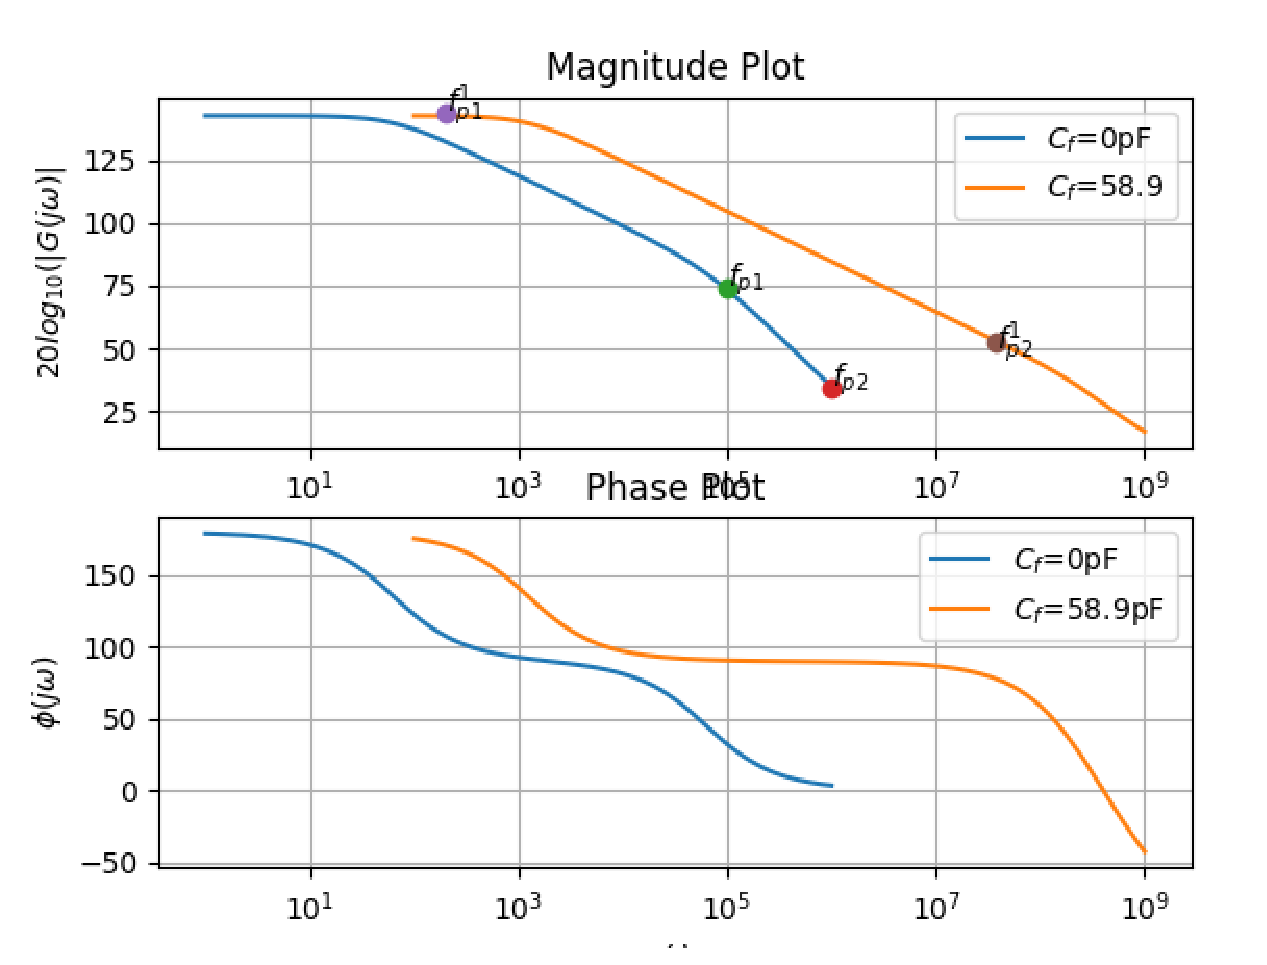
\includegraphics[width=\columnwidth]{./figs/ee18btech11029/feedback.eps}
\caption{}
\label{fig:ee18btech11029_1}
\end{figure}
The presence of $C_{f}$ has the effects

\begin{itemize}
    \item It downshifts the first pole by factor of $\frac{10^{5}}{200}=500$
    \item It upshifts the second pole by factor of $\frac{37.95\times10^{6}}{10^{6}}=37.95$
\end{itemize}
Verify the above plot by
\begin{lstlisting}
codes/ee18btech11029/ee18btech11029_1.py
\end{lstlisting}

\item Design the circuit\\
\solution
\begin{figure}[ht!]
	\begin{center}
		\resizebox{\columnwidth}{!}{\tikzstyle{block} = [draw, rectangle, 
    minimum height=1.25em, minimum width=2.5em]
\tikzstyle{sum} = [draw, circle, node distance=1cm]
\tikzstyle{input} = [coordinate]
\tikzstyle{output} = [coordinate]
\tikzstyle{pinstyle} = [pin edge={to-,thin,black}]


\begin{tikzpicture}[auto, node distance=3.5cm,>=latex']

    \node [input, name=input] {};
    \node [sum, right of=input] (sum) {};
    \node [block, right of=sum] (controller) {$\frac{10^{4}}{\brak{1+\frac{s}{2\pi\times10^{5}}}\brak{1+\frac{s}{2\pi\times10^{6}}}\brak{1+\frac{s}{2\pi\times2\times10^{6}}}}$};
    
   
    \node [output, right of=controller] (output) {};
    \node [block, below of=controller] (measurements) {$1$};

    \draw [draw,->] (input) -- node[pos=0.99] {$+$} node {$V_{s}$} (sum);
    \draw [->] (sum) -- node {$V_{i}$} (controller);
    \draw [->] (controller) -- node [name=y] {$V_{o}$}(output);
    \draw [->] (y) |- (measurements);
    \draw [->] (measurements) -| node[pos=0.99] {$-$} node [near end] {$V_{f}$} (sum);
\end{tikzpicture}
}
	\end{center}
	\caption{}
	\label{fig:ee18btech11029_block}
\end{figure}\\
The transfer function of the opamp is
\begin{align}
   G(s)&= \frac{10^{4}}{\brak{1+\frac{s}{2\pi\times10^{5}}}\brak{1+\frac{s}{2\pi\times10^{6}}}\brak{1+\frac{s}{2\pi\times2\times10^{6}}}}
\end{align}
\item For feedback gain H\\
\solution
The value of the feedback gain is 1,So just place a wire between the input and the output terminal
\begin{align}
    H=\frac{V_{f}}{V_{o}}=1
\end{align}
\item Design the feedback circuit
\begin{figure}[ht!]
	\begin{center}
		\resizebox{\columnwidth}{!}{\input{./figs/ee18btech11029/ee18btech11029_fig1.tex}}
	\end{center}
	\caption{}
	\label{fig:ee18btech11029_fig1}
\end{figure}


































\end{enumerate}
